\documentclass{article}
\usepackage[utf8]{inputenc}

\title{Figures}
\author{Robert Taylor}
\date{July 2018}

\usepackage{natbib}
\usepackage{graphicx}

\begin{document}

\maketitle

\section{Introduction}
Included in this document are several figures that were obtained from gathering data with libSmoldyn packages and compiled with MATLAB files that are included in the repository. Instructions to recreate the figures, as well as recommended factors to consider when trying to make similar measurements will be discussed for each figure and some general considerations for all simulations run.

\subsection{Comments and Considerations for all figures}

As with all simulations, the units and scales used (or not used) have a considerable impact on the simulation. Smoldyn is not written with any particular system of units in mind, thus much freedom is given to the user to determine the units and scale most suitable for the simulation. Keeping with this theme, I have not performed these simulations with any particular length or time scale in mind and consider the the spatial and temporal dimensions to be unitless. For all of the figures below, units will be omitted. If there is a desire to replicate these figures with the intention of applying them to a system where distance and time have explicit units, it is important to make sure to appropriately scale all parameters appropriately, including the world and region size, the Smoldyn time step and end times, the diffusion coefficients, and binding rates and radii.

The time step that is provided to Smoldyn is incredibly important for diffusion and consequently for the chemical reactions that occur in the system. In general, for discrete time simulations we expect the numbers to converge as the time step approaches zero, but decreasing the time step too much becomes computationally expensive and impractical after a certain point. As will be discussed later in the document, the chosen time step can have a drastic effect on equilibrium values of bidirectional chemical reactions , an effect that is not observed in 3d simulations. This inconsistency is only seen in the bimolecular reactions, and is part of our motivation to refer to the probability of a binding event to occur in terms of the reaction radius rather than a specific rate.

\section{Simple MFPT}

Figure 1 provides the collected mean first passage times (MFPT) for various numbers of particles, $N$. The timestep used for the parameter is $dt = .00001$, the world size is $L=3$, the region to be evacuated is a circle in the center of the box with radius $R = 1$, and the diffusion constant is $D=1$. There were 100 runs for each $N$. To recreate this data, one can run the makefile given in SmoldynSimpleMFPT and then run the shell script "nSweepMFPT.sh". This will save the data in the folder "Data/nSweep". The MATLAB script, MFPTdata.m loads the data, finds the MFPT for each run, and then plots the MFPT for each $N$.

Figures 2-4 give several empirical CDFs for the first passage times. This uses the same data as was generated from the "nSweepMFPT.sh" shell script but now presents a CDF instead of simply means with an errorbar. These plots can easily be generated for each $N$ by using the included MATLAB function mfptECDF, which simply loads the data generated from the shell script and applies MATLAB's built in ECDF function to it.

\section{Dimerization}

The shell scripts included in the SmoldynDimerization folder collect data for both time series runs and equilibrium monomerization fractions. The characteristic time for these simulations is approximately 18. Equilibrium fractions can be calculated from an average over a time series, data which can be given from either the decay script or the equilibrium script. The equilibrium output outputs all monomers counted, dimers counted, and number of timesteps used in each line, so to find the monomerization fraction, divide the first column by the third column and then by the total number of possible monomers.

Figure 5 gives the equilibrium monomerization fraction for various binding radii over several orders of magnitude of $k_{off}$. Table 1 takes these values and uses cubic interpolation to find the point where the monomerization fraction is .5 in order to find "equivalent" 2d equilibrium binding rates. Note that these do not scale linearly with the binding radius as they would in 3d and are several orders of magnitude higher than would be estimated from the traditional diffusion-controlled reaction rate, $k = 4 \pi D r_{bind}$.
\begin{figure}[h!]
\centering
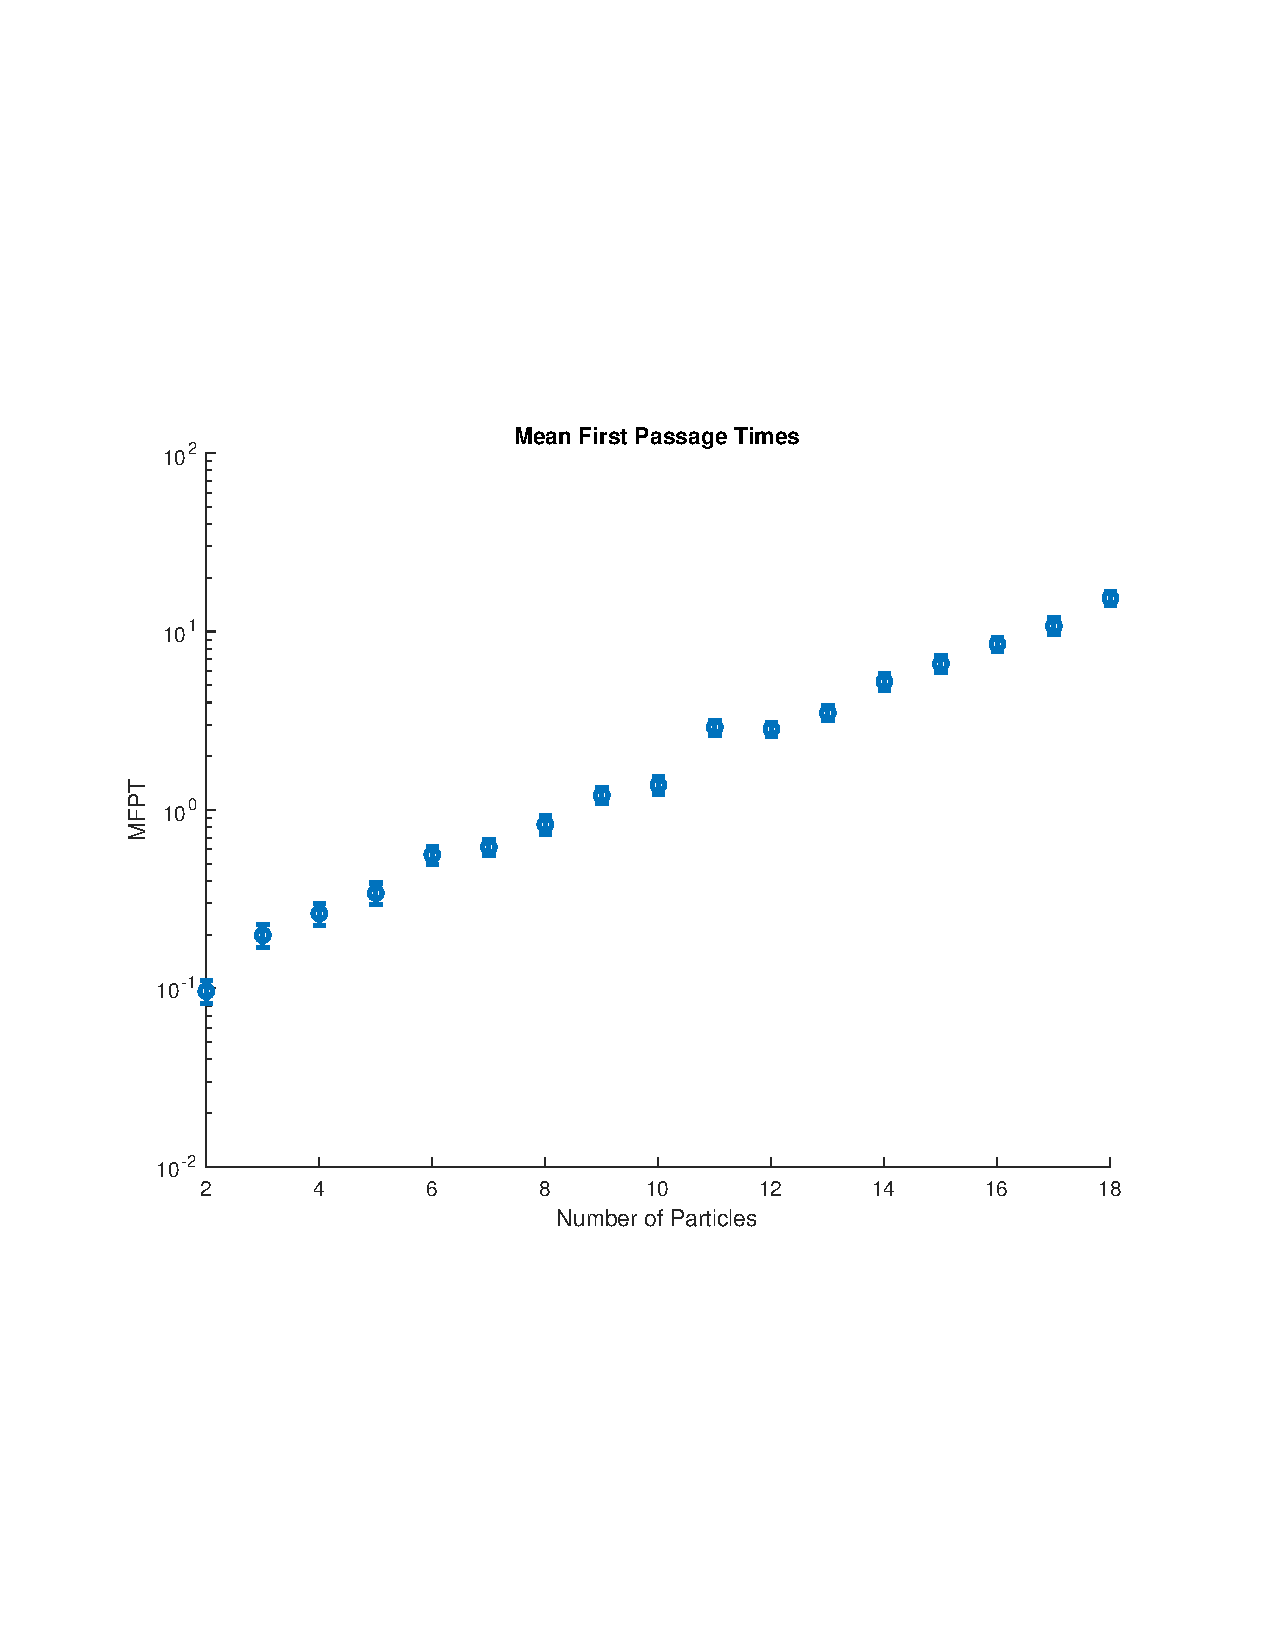
\includegraphics[scale=0.5]{libsmolMFPT.pdf}
\caption{MFPTs for various $N$}
\label{fig:MFPT}
\end{figure}
\begin{figure}[]
\centering
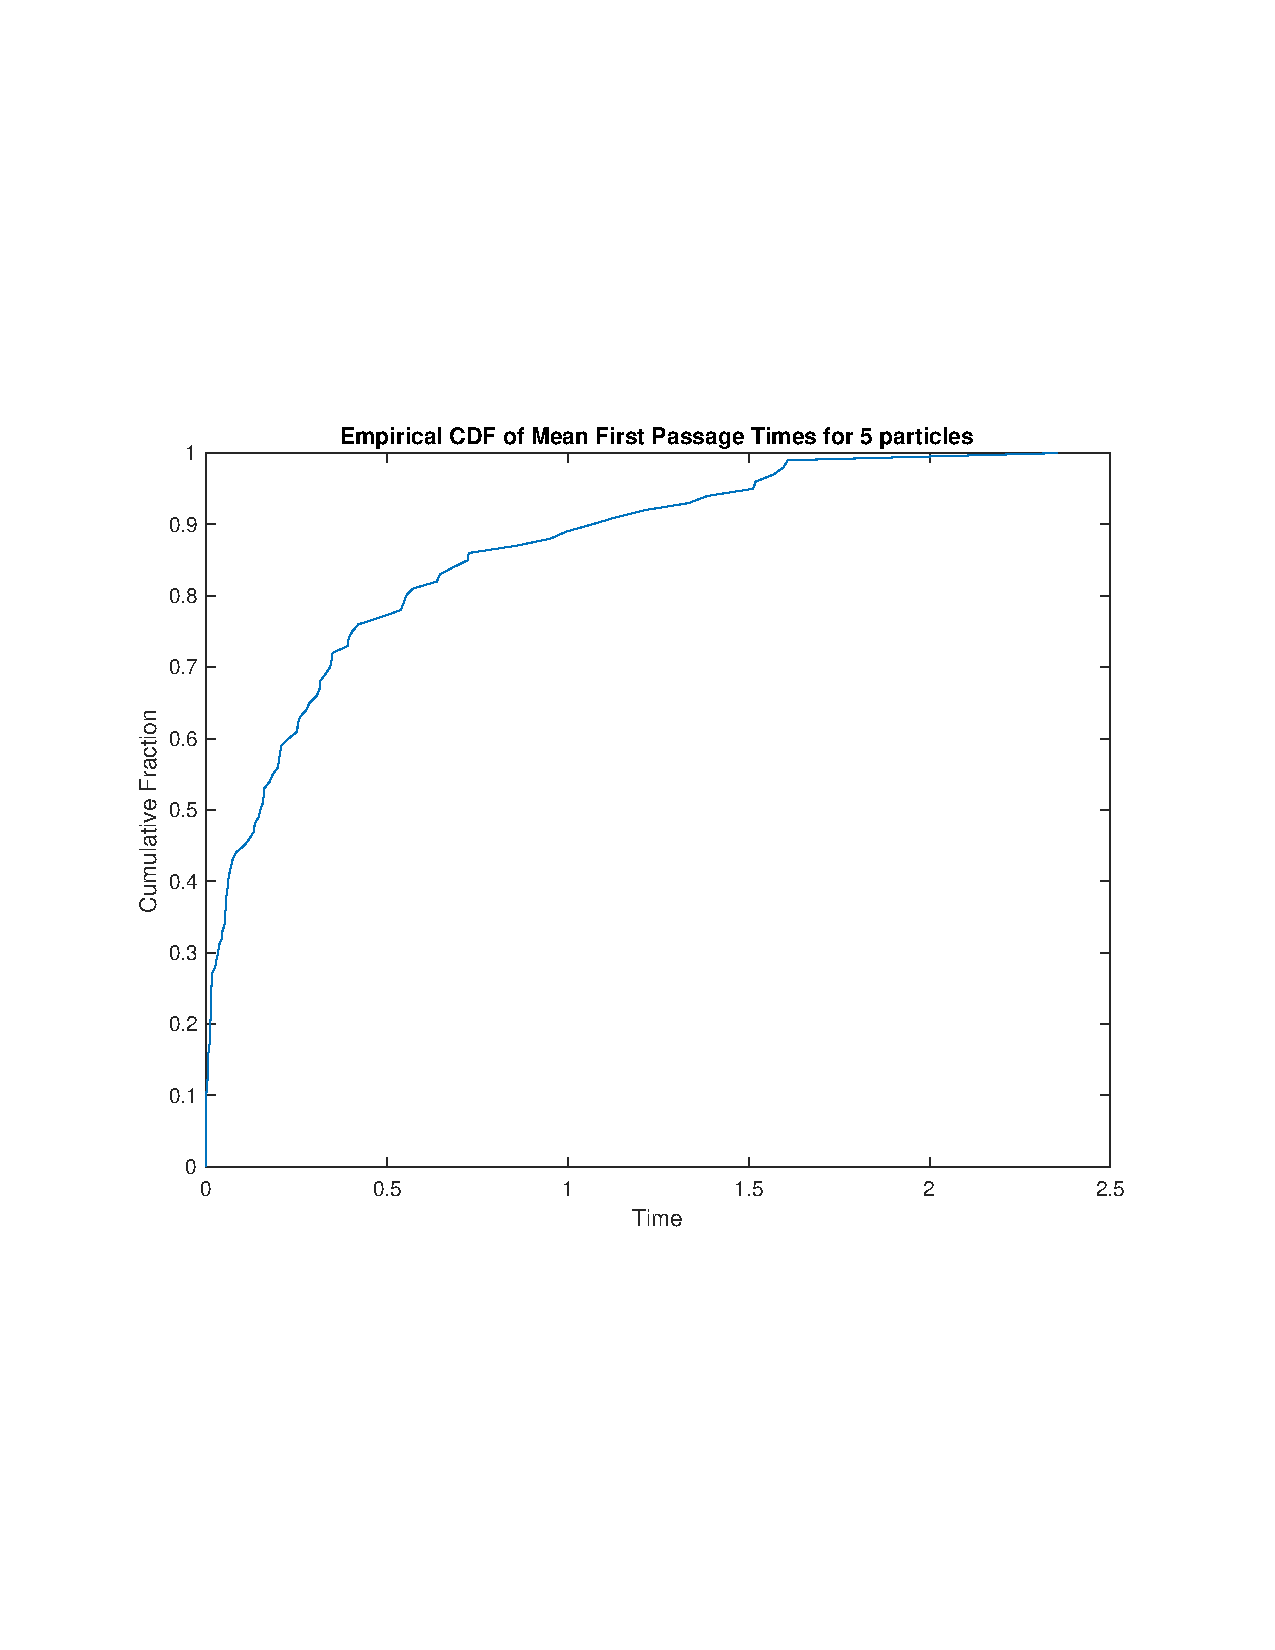
\includegraphics[scale=0.5]{ECDF5.pdf}
\caption{FPT Distribution for $N=5$ particles}
\label{fig:CDF5}
\end{figure}\begin{figure}[]
\centering
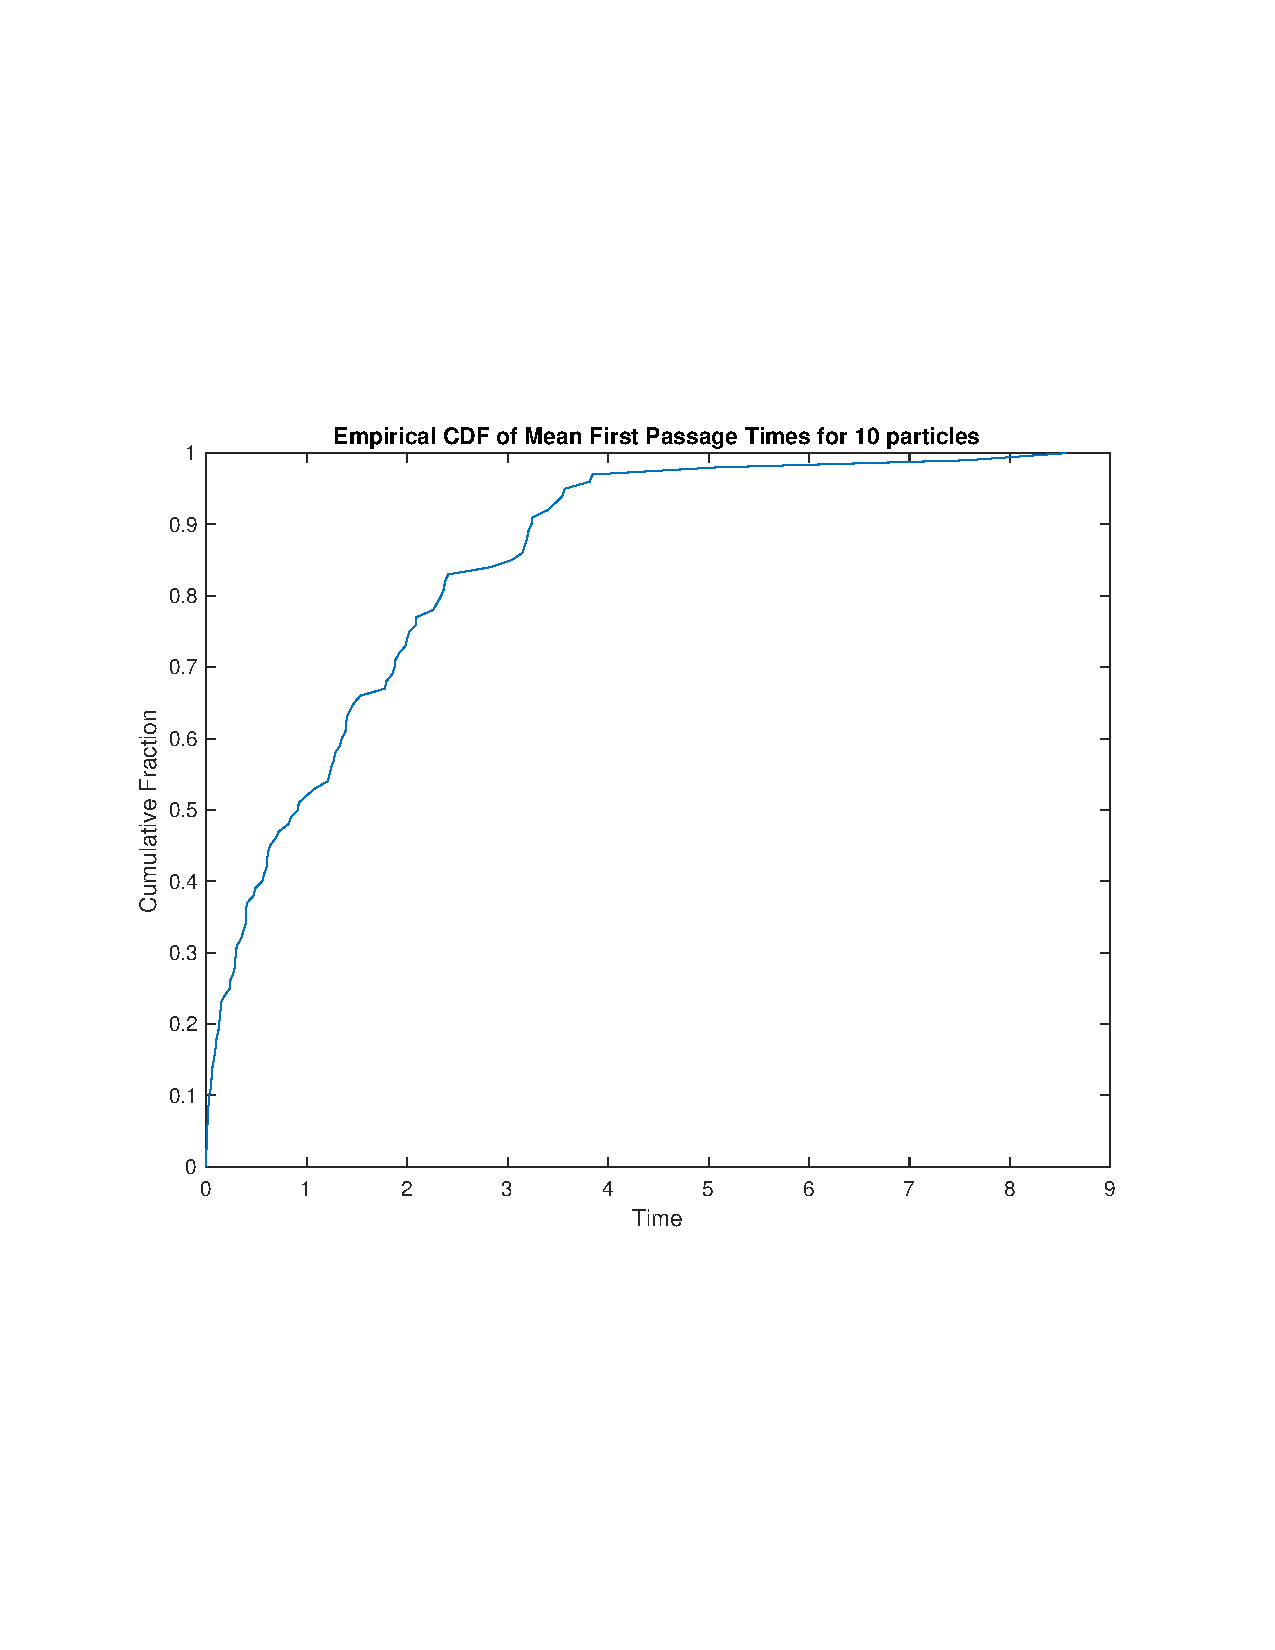
\includegraphics[scale=0.5]{ECDF10.pdf}
\caption{FPT Distribution for $N=10$ particles}
\label{fig:CDF10}
\end{figure}\begin{figure}[]
\centering
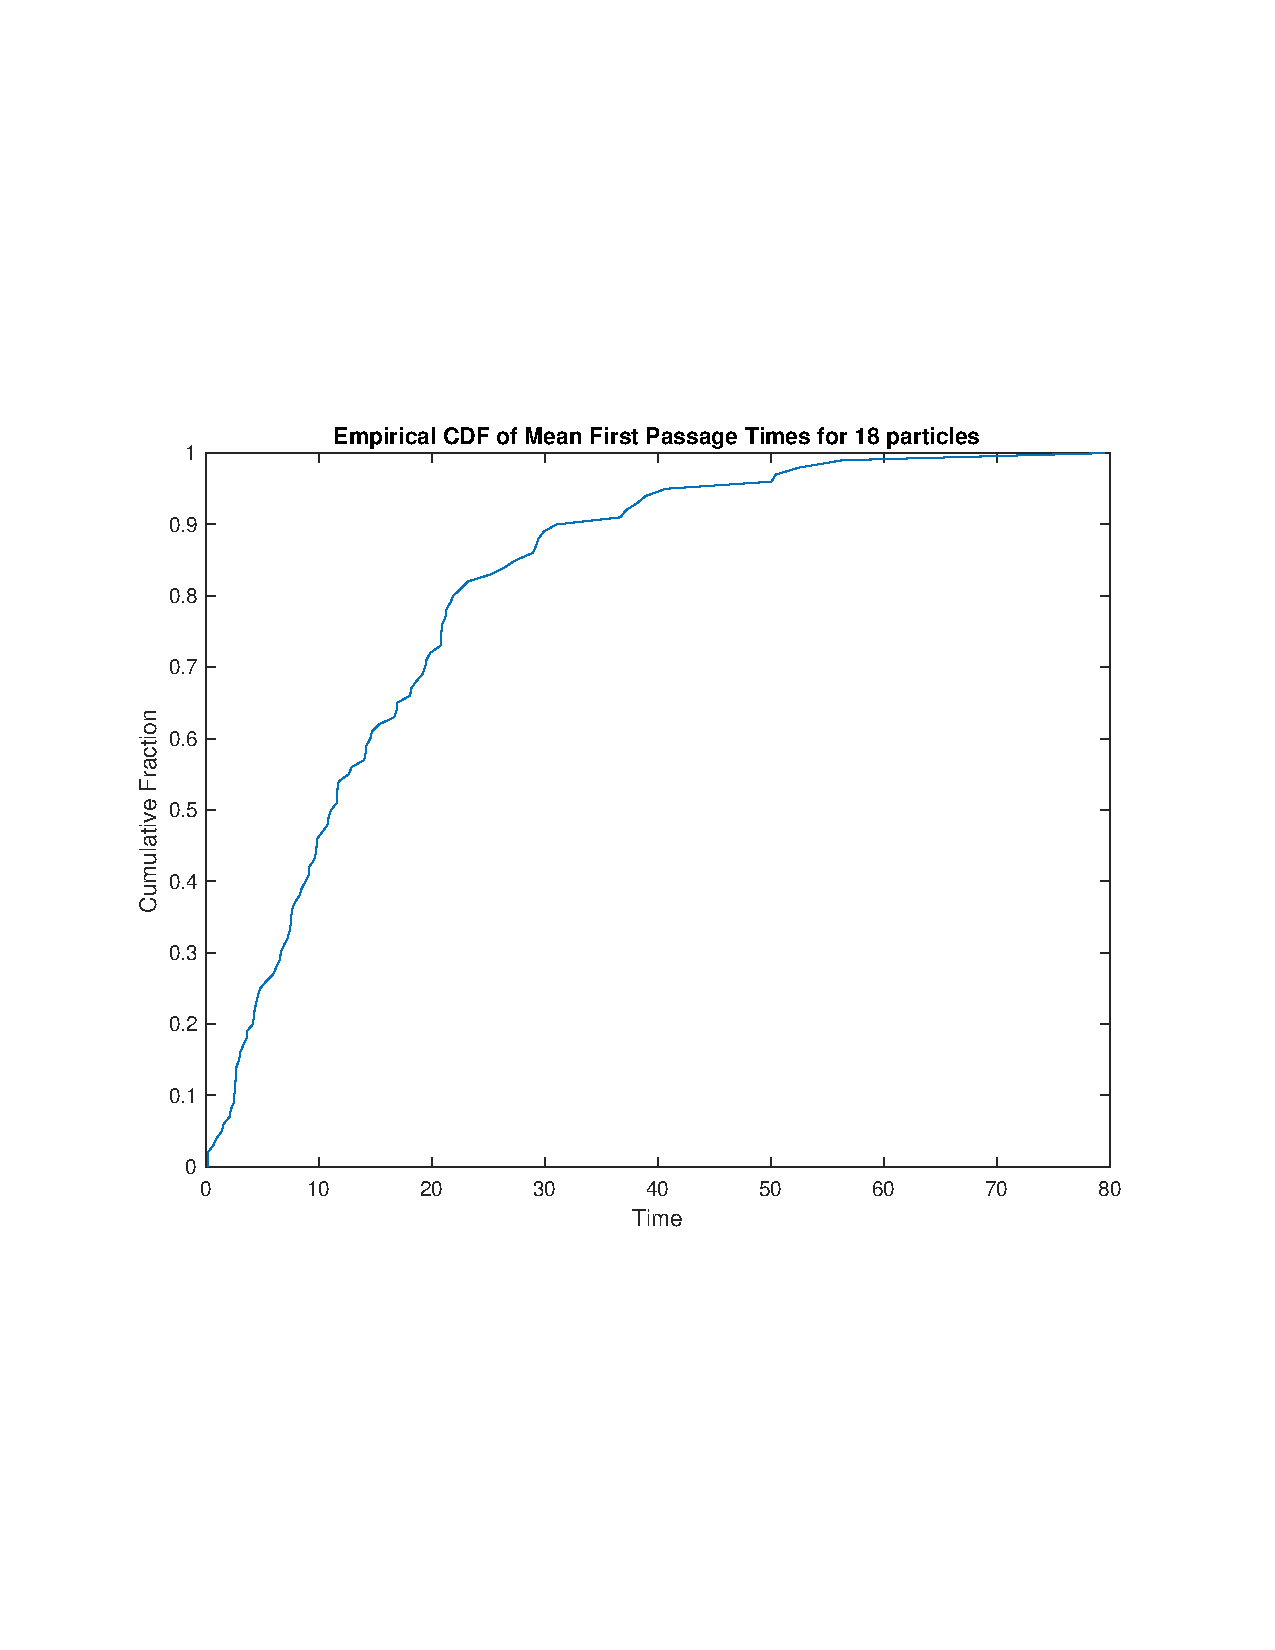
\includegraphics[scale=0.5]{ECDF18.pdf}
\caption{FPT Distribution for $N=18$ particles}
\label{fig:CDF18}
\end{figure}
\begin{figure}[]
\centering
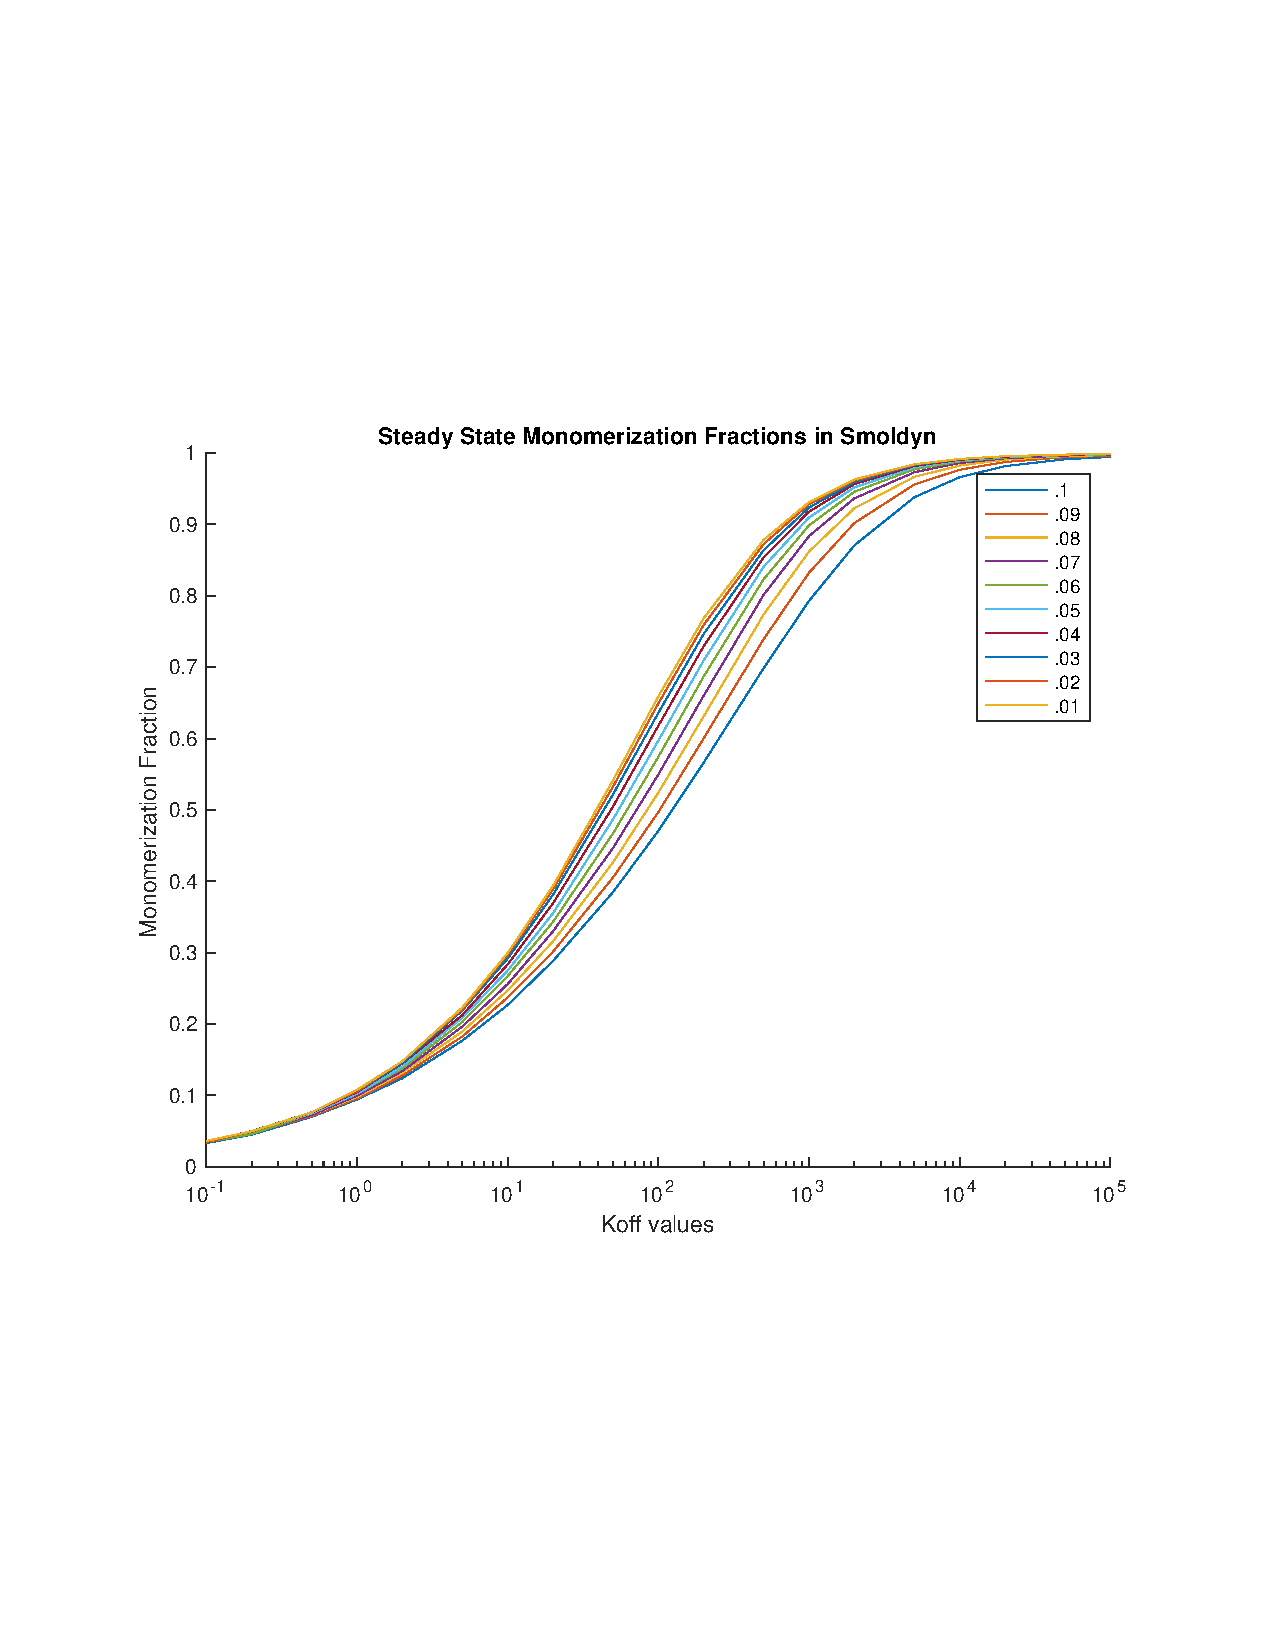
\includegraphics[scale=0.5]{MonomerizationFractions.pdf}
\caption{Equilibrium monomerization fractions for various binding radii. Each curve uses a separate binding radius given by the legend, and the unbinding rates are given by the Koff on the x axis.}
\label{fig:MonomerEquil}
\end{figure}

\begin{table}[]
    \centering

    \begin{tabular}{||c|c||}
    \hline
    $r_{bind}$ & $k_{equiv}$\\
    \hline\hline
         0.01 & 39.43 \\
         0.02 & 41.38 \\
         0.03 & 44.00 \\
         0.04 & 48.65 \\
         0.05 & 54.33 \\
         0.06 & 62.10 \\
         0.07 & 72.23 \\
         0.08 & 84.94 \\
         0.09 & 102.18 \\
         0.10 & 124.22 \\
         \hline
    \end{tabular}
    \caption{Equivalent equilibrium binding rates for various binding radii}
    \label{tab:Kequiv}
\end{table}

\begin{figure}[]
\centering
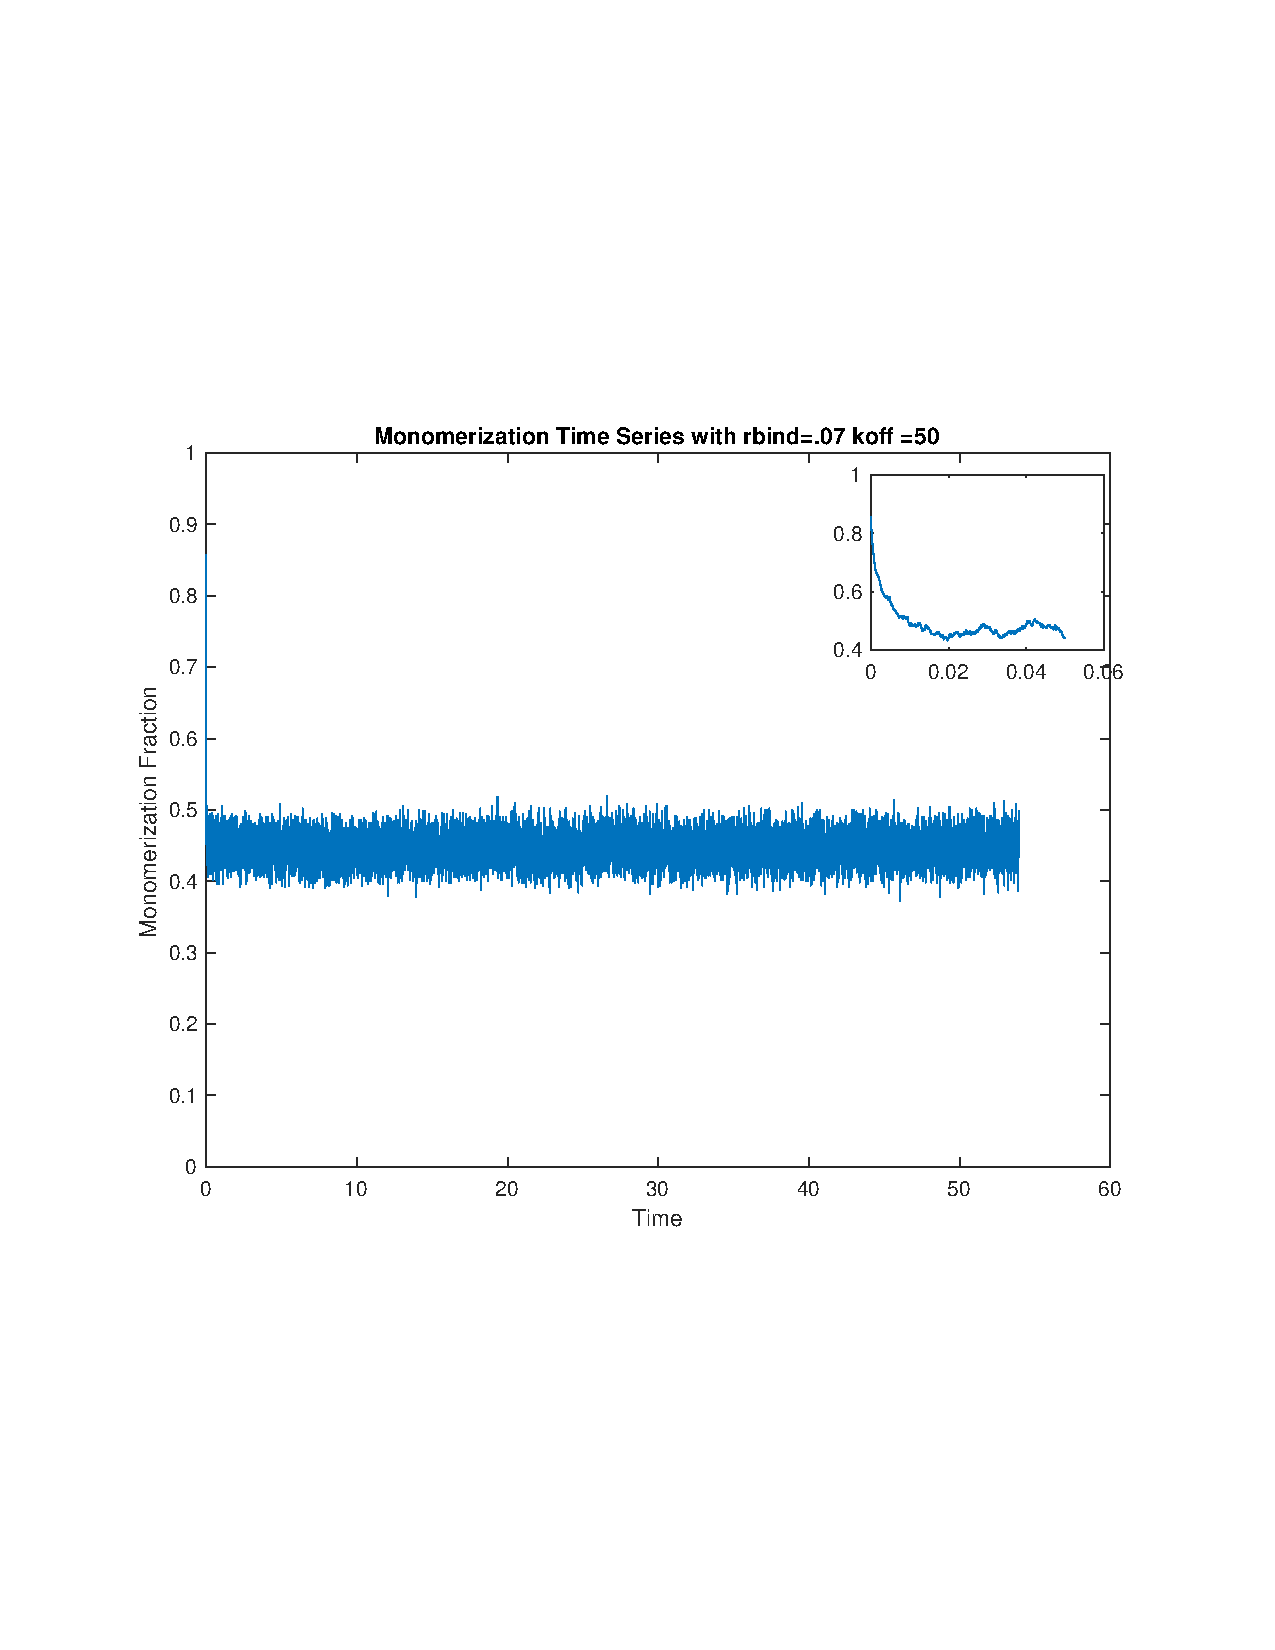
\includegraphics[scale=0.5]{timeSeries.pdf}
\caption{Time series of monomerization fraction. Inset: Time series for first 5000 time steps (.05 units of time)}
\label{fig:timeSeries}
\end{figure}

\end{document}
